
\item In the arrangement of Fig. 1.9 the masses \( m_0 \), \( m_1 \), and \( m_2 \) of bodies are equal, the masses of the pulley and the threads are negligible, and there is no friction in the pulley. Find the acceleration \( w \) with which the body \( m_0 \) comes down, and the tension of the thread binding together the bodies \( m_1 \) and \( m_2 \), if the coefficient of friction between these bodies and the horizontal surface is equal to \( k \). Consider possible cases.
    \begin{center}
        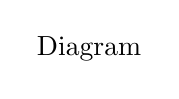
\begin{tikzpicture}
            \node at (0, 0) {Diagram};
        \end{tikzpicture}
    \end{center}


\begin{solution}
    \begin{center}
        \begin{tikzpicture}
            \draw (0,0) rectangle (1,2);
            \draw (1, 2) -- (1,3);
            \draw[->] (1.5, 2.5) -- (2.5, 2.5);
            \draw (2.2,2.2) rectangle (2.7,2.7);
            \draw (2.7, 2.5) -- (3.7,2.5);
            \draw (3.1,2.2) rectangle (3.6,2.7);
            \node at (4,2.5) {k$N_2$};
            \node at (3, 3) {$T_1$};
            \node at (2.3, 2.75) {$N_1$};
            \node at (2, 3) {$T_2$};
            \node at (1.25, 1.5) {T$_1$};
            \node at (1.5, 2.5) {$m_1 g$};
            \node at (3.5, 3) {m$_2 g$};
            \node at (-0.5, 1) {$m_0 g$};
            \draw[thick,->] (0.5,1) --( 0.5, -0.25);
            \node at (-0.75,1){y};
            \node at (1.25,0.05){$N$};
            \node at (-0.75,-1){$ kN_2$};
            \draw[dashed] (0.5,-1) -- (0.5,-2.5); 
        \end{tikzpicture}
    \end{center}
    
    \begin{align*}
        \intertext{Let us write the fundamental equation of dynamics for all the three blocks in terms of projections, having taken the positive direction of $x$ and $y$ axes as shown in the figure and using the fact that kinematical relation between the accelerations is such that the blocks move with same value of acceleration (say $w$)}
        m_0g - T_1 &= m_0w \quad \tag{1}\\
        T_1 - T_2 - km_1g &= m_1w \quad \tag{2}\\
        \intertext{and}
        T_2 - km_2g &= m_2w \quad \tag{3}
        \intertext{The simultaneous solution of Eqs. (1), (2) and (3) yields,}
        w &= g \left[\dfrac{m_0 - k \left( m_1 + m_2 \right)}{m_0 + m_1 + m_2}\right]\\
        \intertext{and}
        T_2 &= \dfrac{(1+k) m_0}{m_0 + m_1 + m_2} m_2g
        \intertext{As the block $m_0$ moves down with acceleration $w$, so in vector form}
        \vec{w} &= \left[\dfrac{m_0-k(m_1+m_2)}{m_0+m_1+m_2}\right]\vec{g}
    \end{align*}
\end{solution}

